\chapter{Stereo recalibration}
\label{cha:stereo_recalibration}

TODO...

* It will be introduced in this chapter the notation and the theory used for the rest of the thesis

* but worked in the stereo and with synthetic data.

* Proposed initializations

* Method selection (triangulation because it is easy to extend for multi-view, and blahblah...).


\section{Theoretical background}
\label{sec:theoretical_background}

\subsection{Pinhole camera model}

A 2D point is denoted by $\mathbf{x} = [x,y]^T$. A 3D point is denoted by $\mathbf{X} = [X,Y,Z]^T$. It is used $\mathbf{\tilde{x}}$ to denote the augmented vector by adding $1$ as the last element: $\mathbf{\tilde{x}} = [x,y,1]^T$ and $\mathbf{\tilde{X}} = [X,Y,Z,1]^T$. A camera is modeled by the usual pinhole: the relationship between a 3D point $\mathbf{X}$ and its image projection $\mathbf{x}$ is given by
\begin{equation}
  s\,\mathbf{\tilde{x}} = K\, [R | t]\,\mathbf{\tilde{X}} \quad \mbox{with } K =
    \begin{pmatrix}
      f_x & 0   & c_x \\
      0   & f_y & c_y \\
      0   & 0   & 1
\end{pmatrix}
\end{equation}

\noindent
where $s$ is an arbitrary scale factor; $(R,t)$ called the extrinsic parameters, is the rotation and translation which relates the world coordinate system to the camera coordinate system; $K$ is called the camera intrinsic matrix, and $(c_x,c_y)$ are the coordinates of the principal point, $f_x$ and $f_y$ are the focal lengths expressed in pixel units.




\subsection{Bundle adjustment}

Needing to estimate relative poses of several cameras or many poses of a single moving camera is a common problem. It is often solved by jointly estimating the set of camera poses along with 3D features that are detected by some set of cameras. This approach is called bundle adjustment (BA) \cite{BA}.

Bundle adjustment algorithms take the following three data as inputs (see Figure~\ref{fig:BA}):
\begin{itemize*}
 \item a set of $n$ 3D point positions $X_1, X_2, \dots, X_n$,
 \item $m$ camera parameters $P_1, P_2, \dots, P_m$,
 \item and the positions of the projections $x_{ij}$ (measurements) of the points $Xi$ in the camera $Pj$ where they are visible.
\end{itemize*}

\begin{figure}[!htbp]
 \centering
 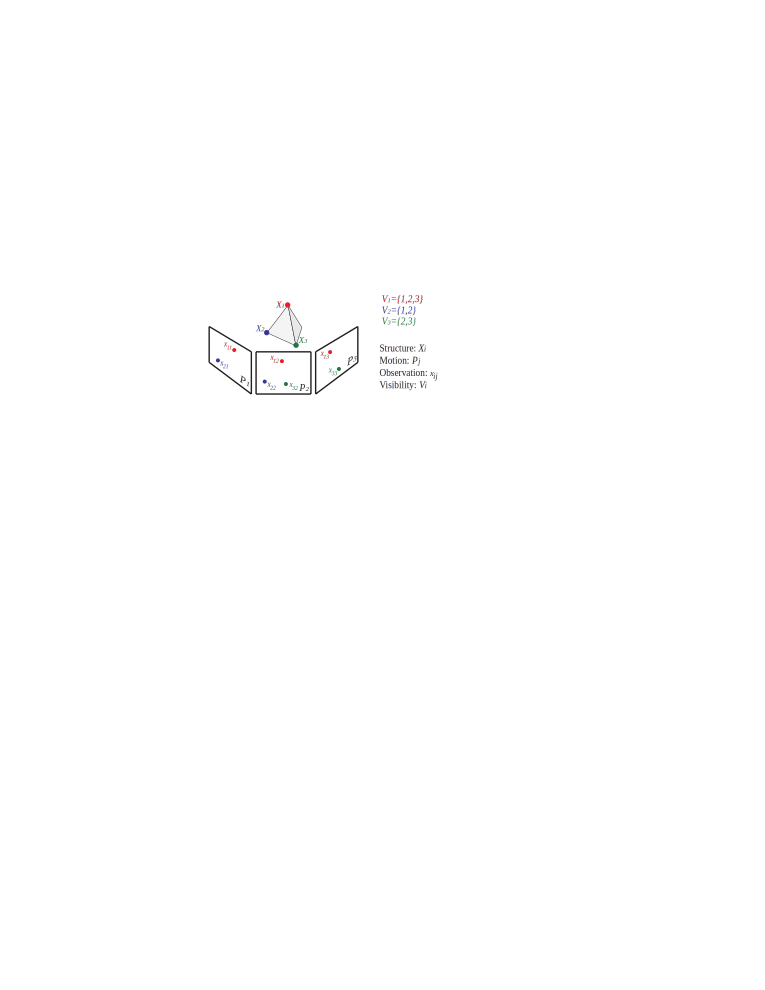
\includegraphics[width=0.45\textwidth]{images/BA.png}
 \caption{Three points $X_1, X_2, X_3$ are observed by three cameras $P_1, P_2, P_3$.}
 \label{fig:BA}
\end{figure}


\subsection{Triangulation}
TODO...

\subsection{Camera resection}
TODO...





\section{Synthetic data}

TODO...


